\documentclass[10pt,a4paper]{article}
\usepackage[utf8]{inputenc}
\usepackage{amsmath}
\usepackage{amsfonts}
\usepackage{amssymb}
\usepackage{graphicx}
\begin{document}
Jose Antonio's Lagrangian 
\begin{eqnarray} 
\mathcal{L} & = & \frac{1}{2}(D^{\mu}\Phi)^{\dagger}D_{\mu}\Phi - \frac{m^2}{2}\Phi^{\dagger}\Phi - \frac{\lambda}{4}(\Phi^{\dagger}\Phi)^2 -\frac{\lambda}{4}v^4   \nonumber\\
 & & +\frac{1}{2}(D^{\mu} \chi)^*D_{\mu} \chi - \frac{m'^2}{2}\chi^*\chi - \frac{\lambda'}{4}(\chi^* \chi)^2 -\frac{\lambda'}{4}v'^4\nonumber \\ 
 & & -\frac{\kappa}{2}\Phi^\dagger\Phi\chi^*\chi  -\frac{\kappa}{2}v^2v'^2 -\frac{1}{4}\mathcal{F}^{\mu\nu}\mathcal{F}_{\mu\nu}, %+ \frac{1}{4}B_{\mu\nu}B_{\mu\nu}
\end{eqnarray}
where 
\begin{eqnarray*}
D_{\mu} \Phi & \equiv & (\partial_{\mu} + ih\mathcal{A}_{\mu})\Phi, \\ 
D_{\mu} \chi & \equiv & (\partial_{\mu} + ih'\mathcal{A}_{\mu})\chi, \\
\mathcal{F}_{\mu\nu} & \equiv & \partial_{\mu}\mathcal{A}_{\nu}-\partial_{\nu}\mathcal{A}_{\mu}.%,\\
%B_{\mu\nu} & = & \partial_{\mu}B_{\nu}-\partial_{\nu}B_{\mu}.
\end{eqnarray*}

In order to explore the profile of the string, we solve the non-linear system of second order differential equations for the fields $\phi$, $\xi$ and $a$ 
\begin{equation}
	\partial_r^2 \phi + \frac{1}{r} \partial_r \phi- \frac{1}{r^2}\left(n^2+2nha+h^2a^2\right)\phi- m^2 \phi- \lambda \phi^3-\kappa \phi \xi^2 = 0,
\end{equation}
\begin{equation}
	\partial_r^2 \xi + \frac{1}{r} \partial_r \xi - \frac{1}{r^2}\left(n'^2+2n'h' a+h'^2a^2 \right)\xi -m'^2\xi - \lambda' \xi^3 - \kappa \xi \phi^2 = 0 ,
\end{equation}
\begin{equation}
	\partial_r^2a -\frac{1}{r}\partial_r a-hn\phi^2-h^2a\phi^2-h' n'\xi^2 - h'^2 a \xi^2 = 0.  
\end{equation}
When $n,n'\neq 0$, they are subject to the boundary conditions,
\begin{eqnarray}
	\phi(0)=0, & \displaystyle\lim_{r\to\infty}\phi(r) = v, \nonumber \\
	 \xi(0)=0, &  \displaystyle\lim_{r\to\infty}\xi(r) = v', \nonumber  \\
	 a(0)=0, & \displaystyle \lim_{r\to\infty}a(r) = -\frac{n}{h}=-\frac{n'}{h'},
\end{eqnarray}
and
\begin{align}
	\label{eq:constraints}
	\lambda>0, \ \ \ \lambda'>0, \ \ \ \kappa^2 < \lambda \lambda',\nonumber \\
	 m^2 = -\kappa v'^2 - \lambda v^2<0,\ \ \ m'^2 = -\kappa v^2 - \lambda' v'^2<0. 
\end{align}


Victor's Lagrangian
\begin{eqnarray} 
	\mathcal{L} & = & (D_{\mu}\Phi)^{\dagger}D_{\mu}\Phi - m^2\Phi^{\dagger}\Phi - \lambda(\Phi^{\dagger}\Phi)^2 \nonumber\\
 & & +(D_{\mu} \chi)^*D_{\mu} \chi - m'^2\chi^*\chi - \lambda'(\chi^* \chi)^2  \nonumber \\ 
 & & +\kappa\Phi^\dagger\Phi\chi^*\chi- \frac{1}{4}\mathcal{F}_{\mu\nu}\mathcal{F}_{\mu\nu}. %+ \frac{1}{4}B_{\mu\nu}B_{\mu\nu}
\end{eqnarray}

%If we redifine Jose Antonio's Lagragian by dividing it by 1/2 we obtain (an overall factor does not change the equations of motion)
%
%\begin{eqnarray} 
%\mathcal{L} & = & (D^{\mu}\Phi)^{\dagger}D_{\mu}\Phi - m^2\Phi^{\dagger}\Phi - \frac{\lambda}{2}(\Phi^{\dagger}\Phi)^2 -\frac{\lambda}{2}v^4   \nonumber\\
% & & +(D^{\mu} \chi)^*D_{\mu} \chi - m'^2\chi^*\chi - \frac{\lambda'}{2}(\chi^* \chi)^2 -\frac{\lambda'}{2}v'^4\nonumber \\ 
% & & -\kappa\Phi^\dagger\Phi\chi^*\chi  -\kappa v^2v'^2 -\frac{1}{2}\mathcal{F}^{\mu\nu}\mathcal{F}_{\mu\nu}. %+ \frac{1}{4}B_{\mu\nu}B_{\mu\nu}
%\end{eqnarray}

It is clear that

\begin{eqnarray*}
 \Phi_{\text{Jose Antonio}}    & = &\sqrt{2}\Phi_{\text{Victor}}\\
 \chi_{\text{Jose Antonio}}    & = &\sqrt{2}\chi_{\text{Victor}}\\
 \kappa_{\text{Jose Antonio}}  & = &-\frac{1}{2}\kappa_{\text{Victor}}\\
 \lambda_{\text{Jose Antonio}} & = &\lambda_{\text{Victor}} \\
 \mathcal{A}_{\text{Jose Antonio}} & = &\mathcal{A}_{\text{Victor}}
\end{eqnarray*}


Victor's paramteres $n = -2,\  h = 0.5,\ n' = -10, h' = 2.5, \lambda=\lambda' = 1,\ v =0.01,\ v' = 2 $.

Using the dictionary above, Jose Antonio's parameters are $n = -2,\  h = 0.5,\ n' = -10, h' = 2.5, \lambda=\lambda' = 1,\ v =0.01\sqrt{2} \approx 0.014,\ v' = 2\sqrt{2}\approx 2.82 $ and $-0.5<\kappa<0.5$.


\begin{figure}
	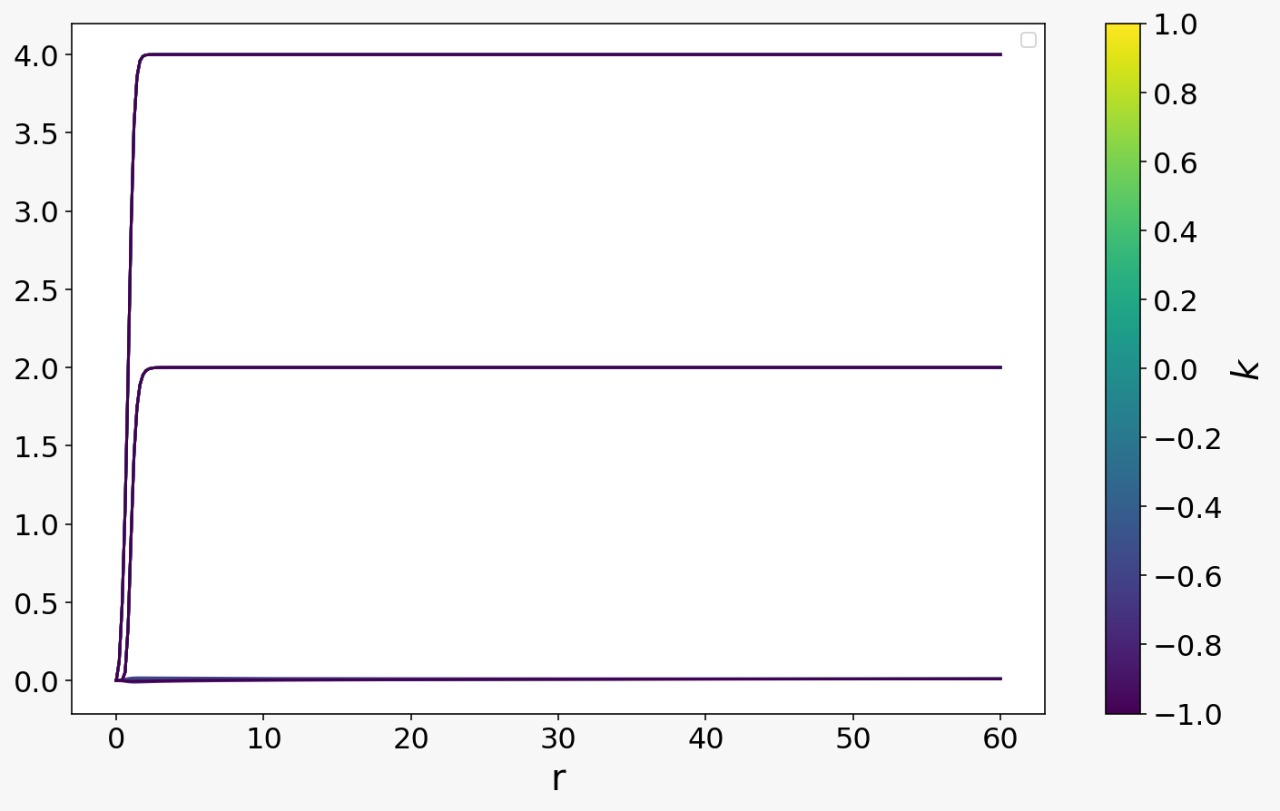
\includegraphics[scale=0.3]{coaxial1.jpeg}
	\caption{Victor's plot: Zoom out}
\end{figure}

\begin{figure}
	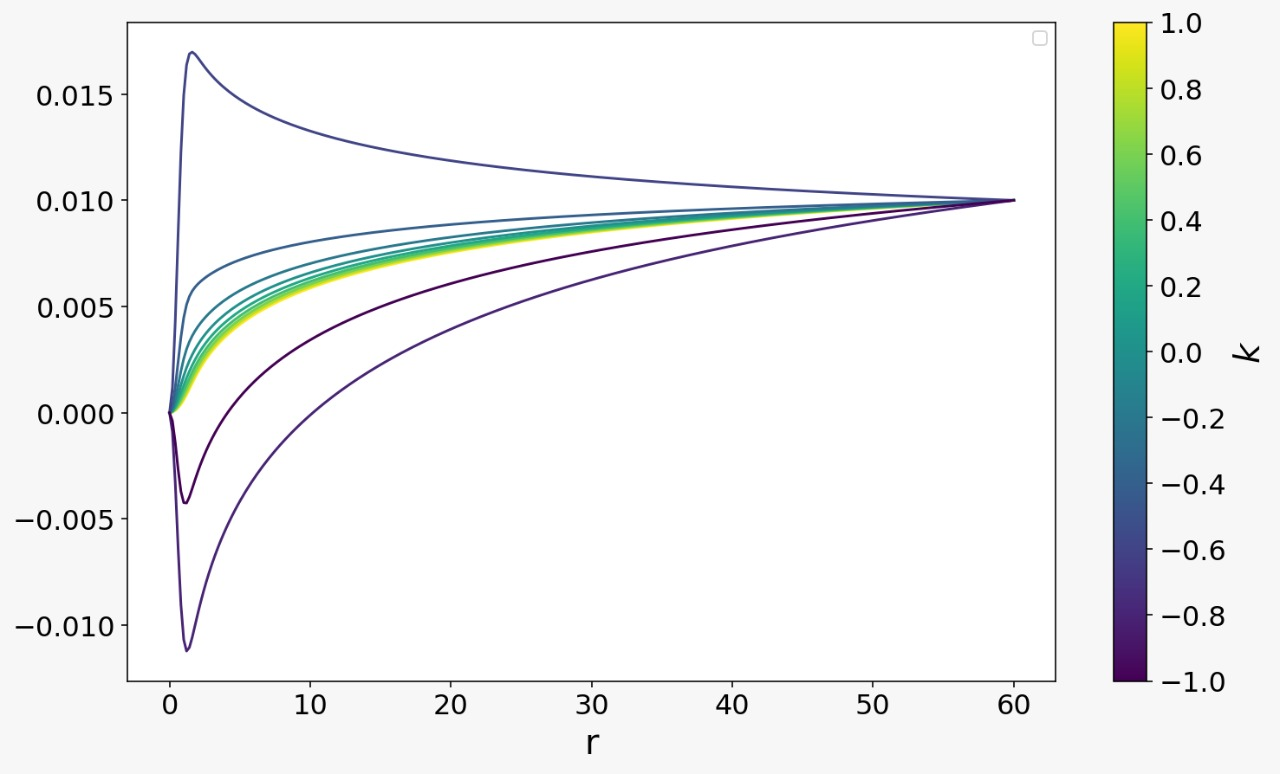
\includegraphics[scale=0.3]{coaxial2.jpeg}
	\caption{Victor's plot: coaxial solution in the $\phi$ field.}
\end{figure}
\begin{figure}
	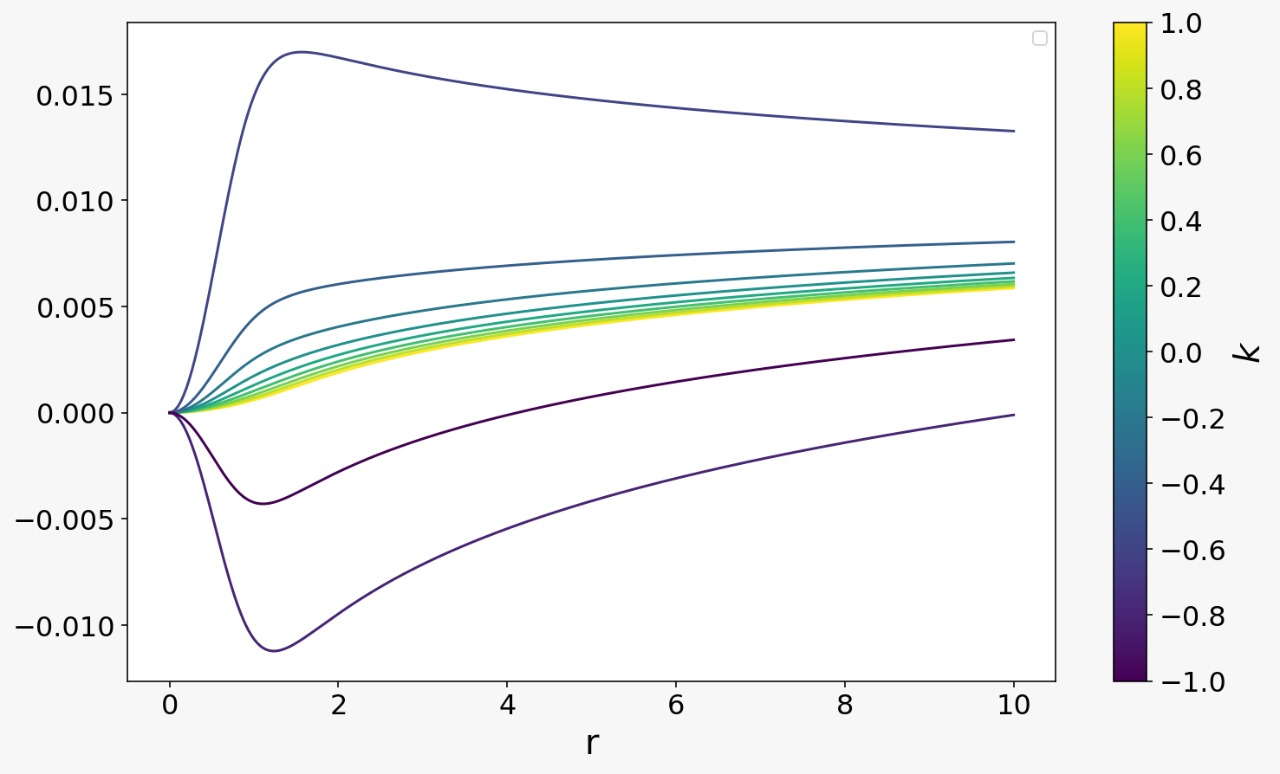
\includegraphics[scale=0.3]{coaxial3.jpeg}
		\caption{Victor's plot: Zoom in, coaxial solution in the $\phi$ field. The coaxial solutions appear when $\kappa = -0.8,\ -1$.}
\end{figure}

\begin{figure}
	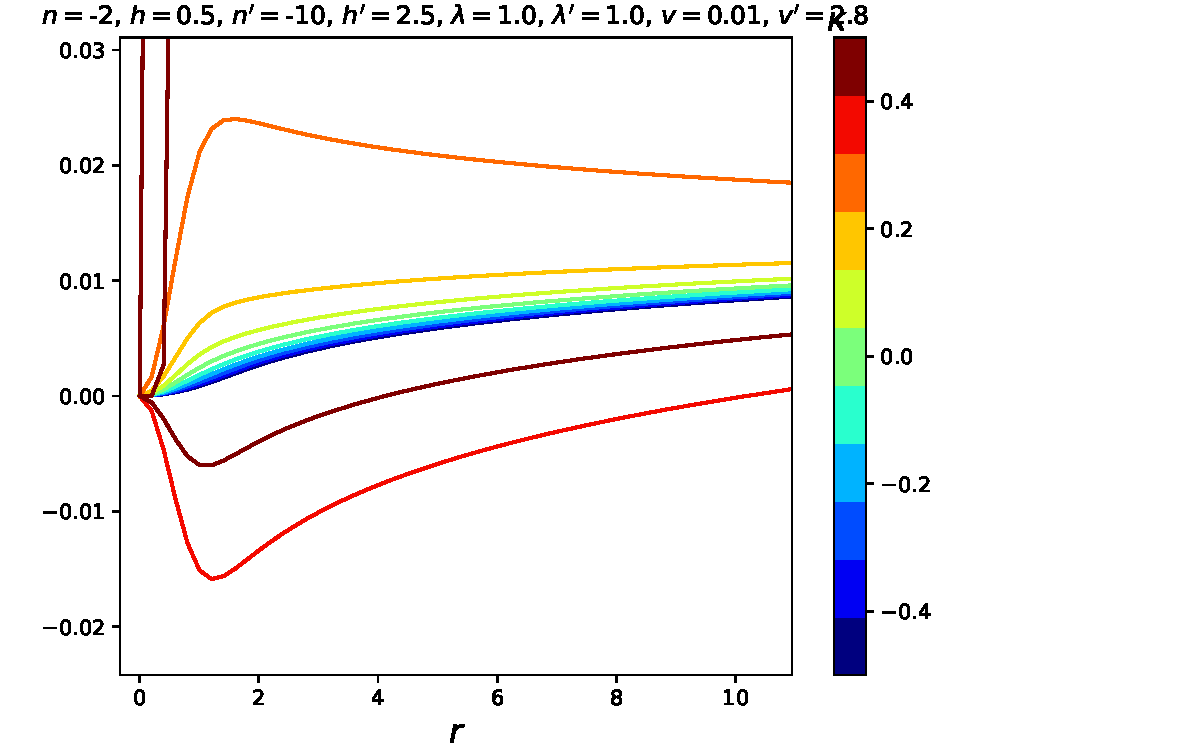
\includegraphics[scale=0.8]{jacoaxialtovicparam.pdf}
	\caption{Jose Antonios's plot: coaxial solution in the field $\phi$.}
\end{figure}

%El modelo estándar posee un simetría global U(1) relacionada a la conservación de la diferencia del número bariónico y leptónico. Al promover esta simetría global a una simetría local, debemos añadir un campo de norma y un neutrino de quiralidad derecha a cada generación de leptones, para cancelar anomalías de norma. Para dar masa al neutrino derecho, agregamos un nuevo campo de Higgs. Las cuerdas cósmicas son defectos topológicos de la configuración de los campos y aparecen como soluciones solitónicas a las ecuaciones de movimiento. Obtuvimos numéricamente el perfil de la cuerda como soluciones a las ecuaciones de movimiento acopladas de los dos campos de Higgs y el campo de norma U(1).

\end{document}